%% =====================================================================
% --- CAPITOLO 7: ARTEFATTI E PROCESSO DI SVILUPPO ---
% =====================================================================
\chapter{Artefatti e Processo di Sviluppo}
\label{cap:artefatti}
% Riferimento Traccia: "Output: Artefatti Software e documentazione del processo di sviluppo"

Questo capitolo descrive gli artefatti tecnici prodotti e i processi utilizzati per la gestione del codice sorgente, la qualità e il deployment.

\section{Strumenti di Versioning e CI/CD: GitHub}

Per la gestione del codice sorgente e il versionamento del progetto, il team ha scelto di utilizzare GitHub. GitHub è una piattaforma di hosting basata sul sistema di controllo versione distribuito Git. Essa non si limita a fungere da archivio remoto per il codice, ma offre un ecosistema completo per il social coding, integrando strumenti per la gestione delle issue, la revisione del codice (Code Review) e l'automazione dei flussi di lavoro (CI/CD). La scelta di GitHub ha permesso di centralizzare lo sviluppo, garantendo un punto di riferimento unico e sincronizzato per tutti i membri del gruppo.

\subsection{Organizzazione dei Repository}
Per garantire una netta separazione delle responsabilità e facilitare lo sviluppo parallelo, il team ha adottato una strategia a \textbf{due repository distinti}:

\begin{itemize}
    \item \textbf{Repository Frontend:} Contiene il codice sorgente dell'interfaccia utente, una Single-Page Application (SPA) sviluppata con \textbf{Angular} e \textbf{TypeScript}. Include componenti UI, servizi per la comunicazione con le API, moduli di routing, template HTML e fogli di stile. La separazione permette di gestire autonomamente le dipendenze Angular (Leaflet, FullCalendar, ngx-quill, RxJS) e le configurazioni di build specifiche per il deployment del client.
    
    \item \textbf{Repository Backend:} Contiene il codice del server \textbf{Node.js/Express} scritto in TypeScript, le API REST, la logica di business, lo schema del database (Drizzle ORM) e le configurazioni per PostgreSQL con PostGIS. Include inoltre il Dockerfile per la containerizzazione e i file di configurazione per l'integrazione con servizi esterni (AWS S3, Nodemailer).
\end{itemize}

Questa architettura a repository multipli (multi-repo) offre diversi vantaggi operativi:
\begin{itemize}
    \item \textbf{Isolamento delle dipendenze:} Le librerie frontend (Angular, RxJS) e backend (Express, Drizzle) rimangono separate, evitando conflitti di versione.
    \item \textbf{Pipeline CI/CD dedicate:} Ogni repository dispone della propria GitHub Action, permettendo build e deploy indipendenti.
    \item \textbf{Cicli di rilascio autonomi:} È possibile aggiornare il frontend senza necessità di ridistribuire il backend e viceversa.
    \item \textbf{Ownership chiara:} La separazione facilita l'assegnazione delle responsabilità e la gestione dei permessi di accesso.
\end{itemize}

\begin{figure}[H]
    \centering
    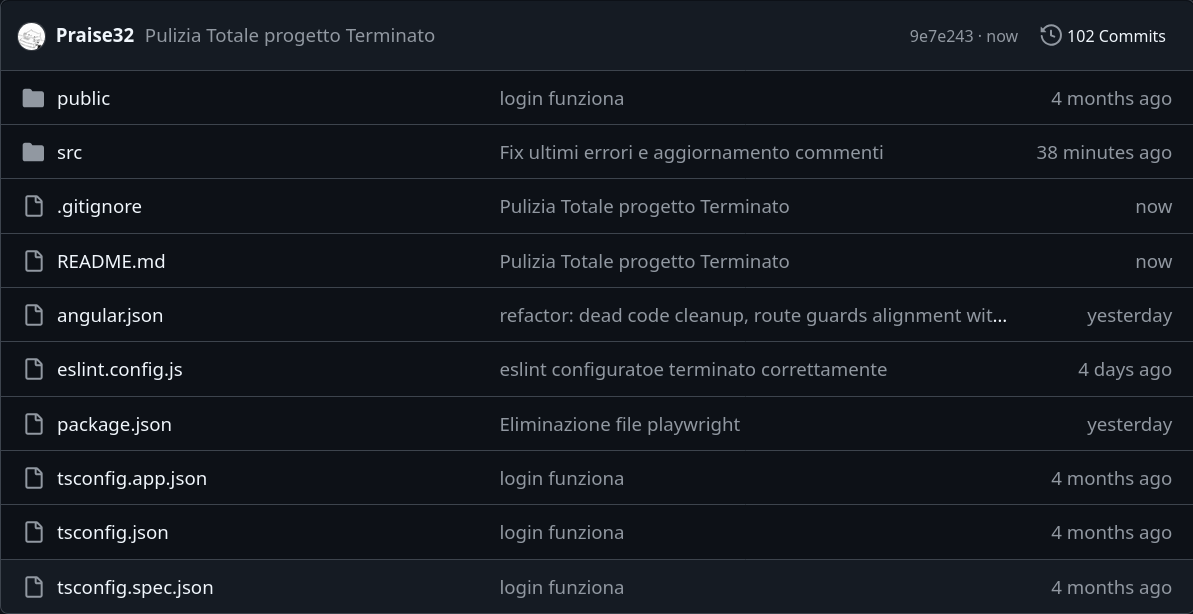
\includegraphics[width=0.9\textwidth]{images/RepoFrontEnd.png}
    \caption{Repository GitHub per il Frontend (Angular)}
    \label{fig:RepoFrontEnd}
\end{figure}

\begin{figure}[H]
    \centering
    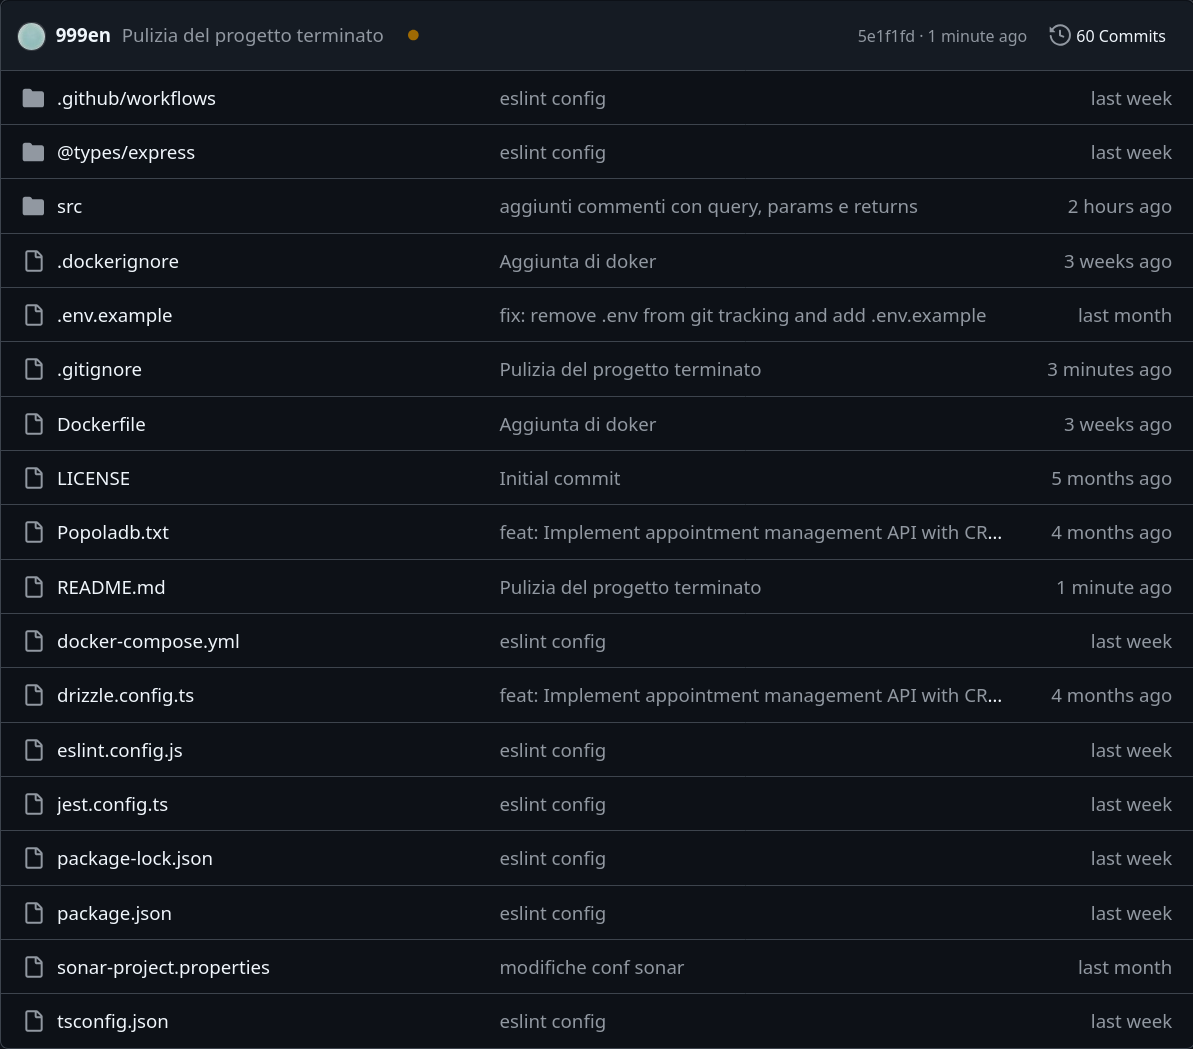
\includegraphics[width=0.9\textwidth]{images/RepoBackEnd.png}
    \caption{Repository GitHub per il Backend (Node.js/Express)}
    \label{fig:RepoBackEnd}
\end{figure}

\subsection{Vantaggi dell'adozione di GitHub}
L'utilizzo di GitHub come strumento di versioning ha apportato benefici tangibili al flusso di lavoro del team, in particolare:

\begin{itemize}
    \item \textbf{Collaborazione facilitata:} GitHub ha permesso al team di lavorare in parallelo su diverse 
    funzionalità senza conflitti bloccanti. Attraverso l'uso dei branch (ramificazioni), ogni sviluppatore 
    ha potuto isolare il proprio ambiente di sviluppo per lavorare su feature specifiche o bugfix. 
    L'integrazione delle modifiche nel ramo principale (main/master) è avvenuta tramite Pull Requests (PR), 
    un meccanismo che ha facilitato la discussione sulle modifiche e la Code Review prima del merge definitivo, 
    migliorando la qualità complessiva del codice.

    \item \textbf{Tracciamento delle modifiche:} La piattaforma offre una visibilità granulare su ogni singola 
    modifica apportata al progetto. Grazie alla cronologia dei commit, è possibile identificare esattamente 
    "chi ha fatto cosa e quando". Questo livello di trasparenza è fondamentale non solo per monitorare 
    l'avanzamento dei lavori, ma anche per il debugging, permettendo di risalire rapidamente all'origine 
    di eventuali errori introdotti nel codice.

    \item \textbf{Ritorno a versioni precedenti (Rollback):} Uno dei vantaggi critici di un sistema di 
    versioning robusto è la possibilità di viaggiare nel tempo all'interno del progetto. In caso di 
    aggiornamenti che introducono regressioni o errori critici, GitHub permette di ripristinare rapidamente 
    lo stato del software a una versione precedente, stabile e funzionante. Questo garantisce una 
    "rete di sicurezza" continua durante tutto il ciclo di sviluppo.

    \item \textbf{Backup e sicurezza:} Essendo un sistema distribuito, il codice risiede sia localmente 
    sulle macchine degli sviluppatori sia sul repository remoto nel cloud di GitHub. Questa ridondanza 
    funge da backup automatico: anche in caso di guasto hardware di un computer locale, il lavoro non 
    viene perso ed è immediatamente recuperabile dal server remoto. Inoltre, GitHub permette di gestire 
    i permessi di accesso, proteggendo il ramo principale da modifiche non autorizzate o accidentali.
\end{itemize}

\begin{figure}[H]
    \centering
    \begin{subfigure}[b]{0.48\textwidth}
        \centering
        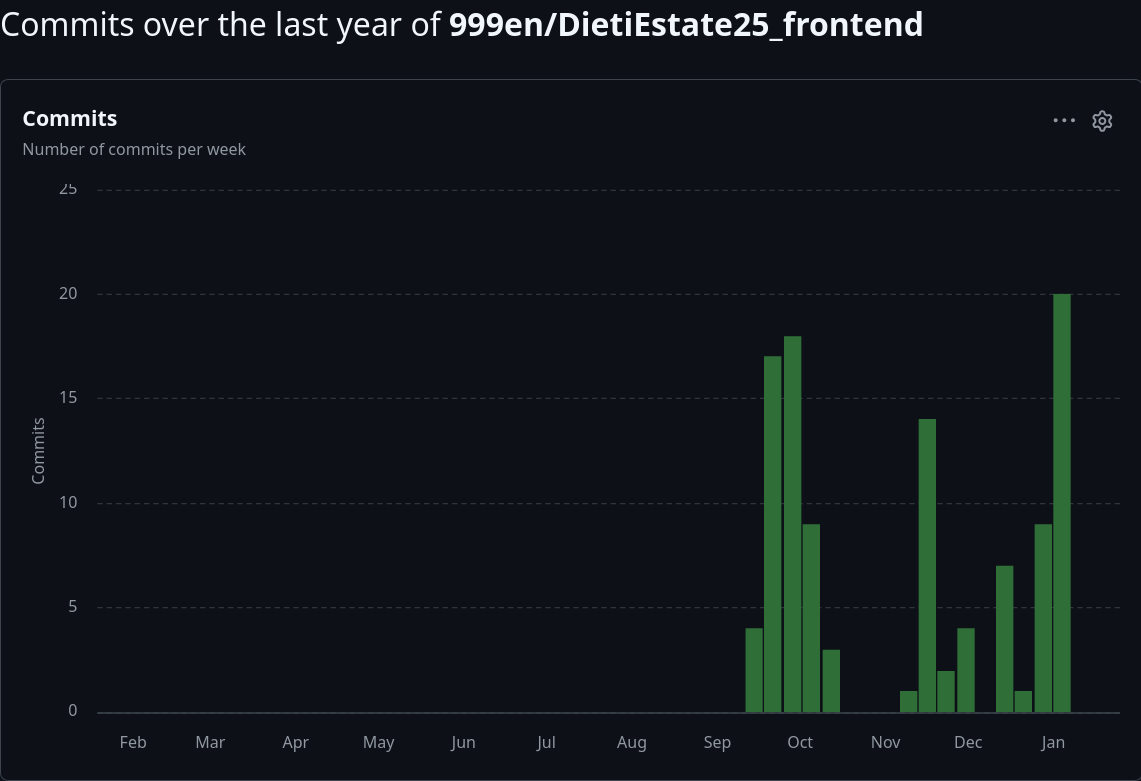
\includegraphics[width=\textwidth]{images/Commits_Frontend.png}
        \caption{Frontend}
        \label{fig:Commits_Frontend}
    \end{subfigure}
    \hfill
    \begin{subfigure}[b]{0.48\textwidth}
        \centering
        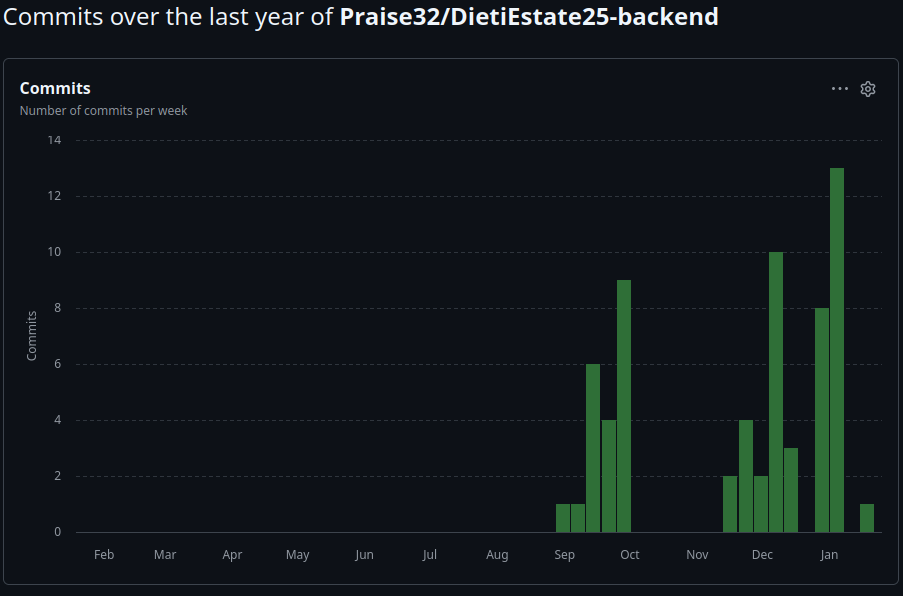
\includegraphics[width=\textwidth]{images/Commits_Backend.png}
        \caption{Backend}
        \label{fig:Commits_Backend}
    \end{subfigure}
    \caption{Grafici dei commit per i repository}
    \label{fig:Commits_Graphs}
\end{figure}

\begin{figure}[H]
    \centering
    \begin{subfigure}[b]{0.48\textwidth}
        \centering
        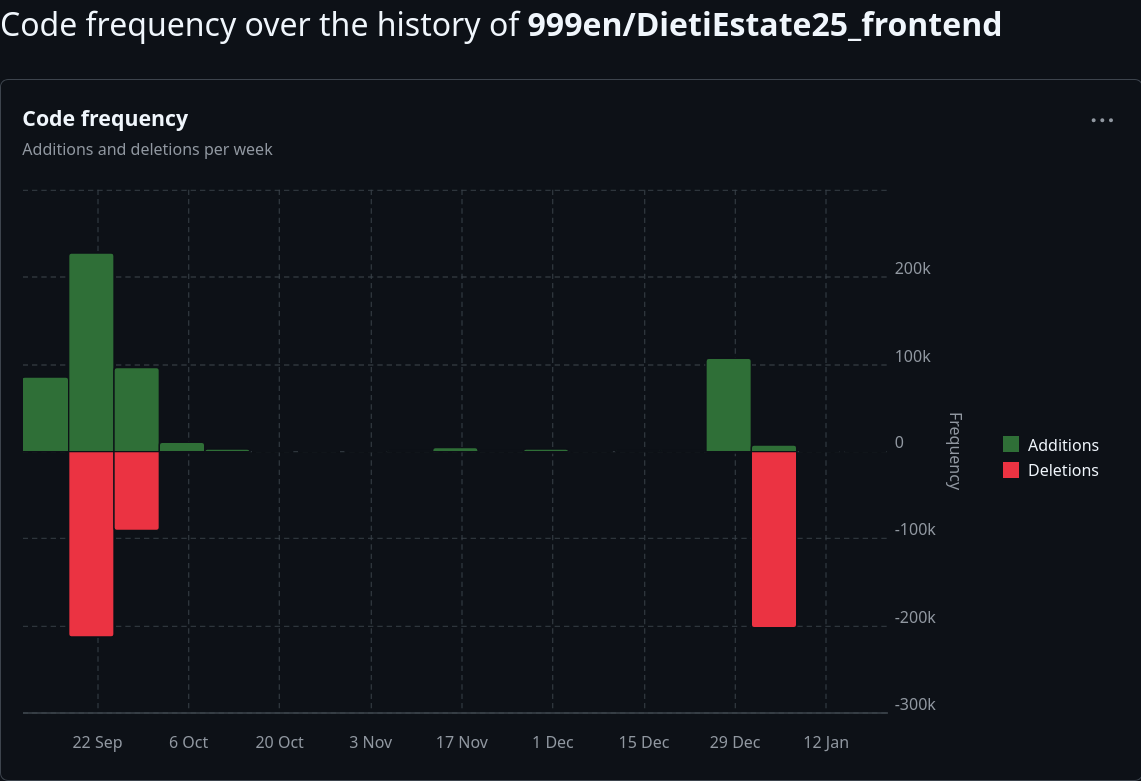
\includegraphics[width=\textwidth]{images/CodeFrequency_Frontend.png}
        \caption{Frontend}
        \label{fig:CodeFrequency_Frontend}
    \end{subfigure}
    \hfill
    \begin{subfigure}[b]{0.48\textwidth}
        \centering
        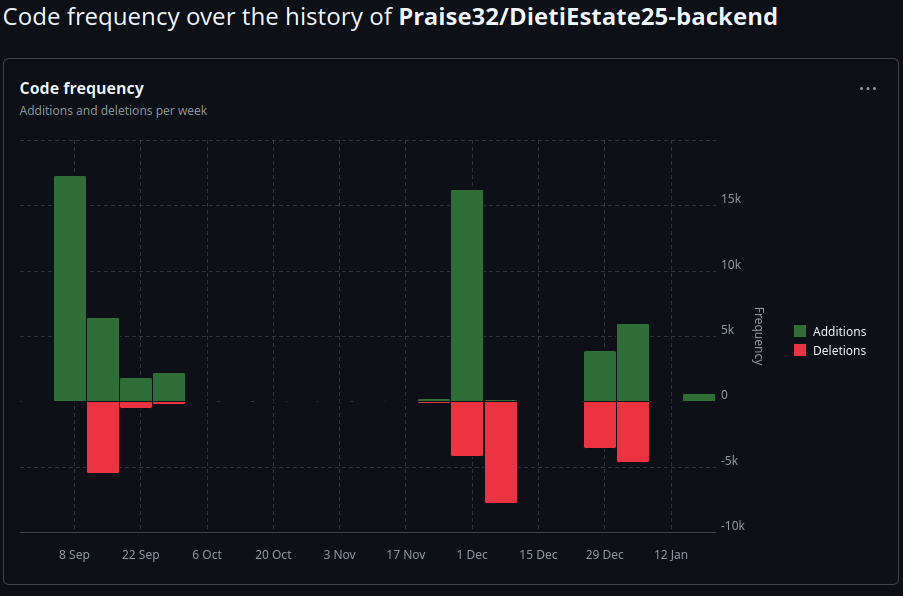
\includegraphics[width=\textwidth]{images/CodeFrequency_Backend.png}
        \caption{Backend}
        \label{fig:CodeFrequency_Backend}
    \end{subfigure}
    \caption{Frequenza delle modifiche (Code Frequency)}
    \label{fig:CodeFrequency_Graphs}
\end{figure}

\subsection{Continuous Integration/Continuous Deployment (CI/CD)}
Oltre al versionamento, il progetto sfrutta le \textbf{GitHub Actions} per automatizzare il ciclo di vita del software. È stata configurata una pipeline di CI/CD che viene eseguita ad ogni \textit{push} sul repository.
La pipeline esegue automaticamente:
\begin{itemize}
    \item \textbf{Installazione delle dipendenze:} Verifica che l'ambiente sia riproducibile.
    \item \textbf{Linting e Type Checking:} Esegue ESLint e il compilatore TypeScript per rilevare errori statici.
    \item \textbf{Testing Automatizzato:} Esegue la suite di test (Jest) per garantire che le nuove modifiche non introducano regressioni.
\end{itemize}
Solo se tutti i passaggi della pipeline hanno esito positivo, il codice è considerato valido per il merge.


\section{Report di Qualità del Codice (SonarQube)}
La qualità del software non si misura solo attraverso il corretto funzionamento delle funzionalità, 
ma anche tramite la struttura interna del codice sorgente. Adottare standard elevati di Clean Code 
è essenziale per garantire la sostenibilità del progetto: un codice pulito riduce il debito tecnico, 
accelera l'inserimento di nuovi sviluppatori e semplifica le future fasi di manutenzione ed evoluzione, 
minimizzando il rischio di regressioni.

\begin{figure}[H]
    \centering
    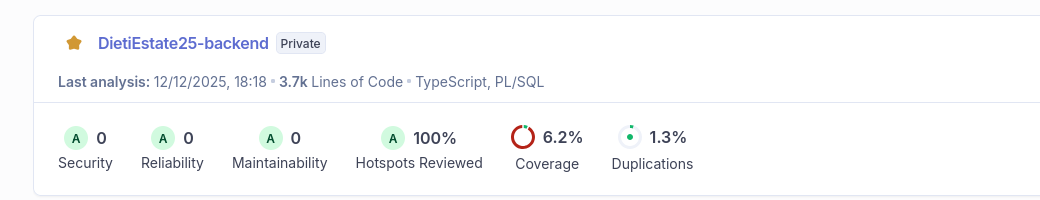
\includegraphics[width=0.8\textwidth]{images/Sonar1.png}
    \caption{Report di qualità del codice con SonarQube }
    \label{fig:Sonar1}
\end{figure}



\subsection{Analisi Statica con SonarQube}
Per oggettivare la qualità del software prodotto, il team ha integrato nel flusso di sviluppo SonarQube, una piattaforma di analisi statica automatizzata. Questo strumento esegue una scansione continua del codice, evidenziando le aree critiche e fornendo metriche precise per guidare le attività di refactoring.

L'analisi si è focalizzata sulle seguenti metriche chiave:

\begin{itemize}
    \item \textbf{Bugs (Affidabilità):} Identificano errori di logica o di programmazione che porteranno quasi sicuramente a un malfunzionamento o a un crash dell'applicazione in fase di esecuzione. La loro risoluzione ha priorità massima per garantire la stabilità del sistema.

    \item \textbf{Vulnerabilità (Sicurezza):} Segnalano punti deboli nel codice che potrebbero essere sfruttati da attacchi esterni (come Injection o esposizione di dati sensibili). Monitorare questo indice è cruciale per garantire la sicurezza dei dati e l'integrità del sistema.

    \item \textbf{Code Smells (Manutenibilità):} Non si tratta di errori bloccanti, ma di violazioni delle buone pratiche di programmazione (es. classi troppo grandi, complessità ciclomatica elevata, nomi di variabili poco chiari). Se trascurati, rendono il codice difficile da leggere e modificare, aumentando i costi di manutenzione futuri.

    \item \textbf{Duplicazioni (Ridondanza):} Rilevano blocchi di codice identici ripetuti in più punti (violazione del principio DRY - Don't Repeat Yourself). Le duplicazioni sono pericolose perché richiedono che ogni modifica venga replicata manualmente in tutti i punti, aumentando il rischio di errore umano.
\end{itemize}

\begin{figure}[H]
    \centering
    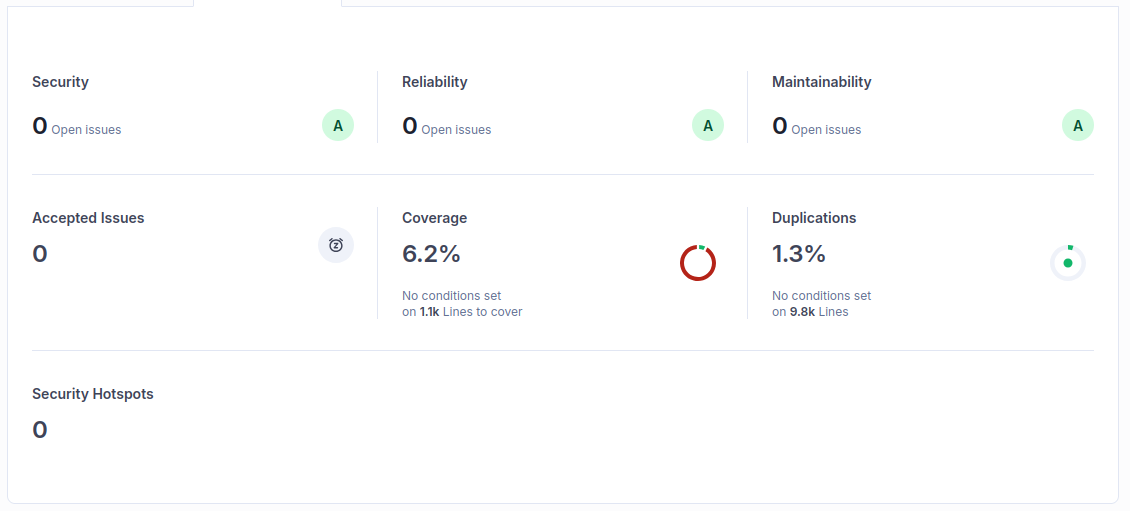
\includegraphics[width=0.8\textwidth]{images/Sonar2.png}
    \caption{Dashboard di SonarQube per il monitoraggio della qualità del codice}
    \label{fig:Sonar2}
\end{figure}

\section{Containerizzazione (Docker)}
% Riferimento Traccia: "Codice Sorgente sviluppato, comprensivo di eventuale Dockerfile."
% Riferimenti Slide: 24 - Virtualizzazione e Cloud.pdf
Il backend è stato containerizzato tramite \textbf{Docker} per garantire portabilità e riproducibilità. È stata adottata una strategia di \textbf{Multi-stage build} per ottimizzare le dimensioni dell'immagine finale e migliorare la sicurezza.

Il processo si divide in due stadi:
\begin{enumerate}
    \item \textbf{Builder Stage:} Utilizza un'immagine Node completa per installare tutte le dipendenze e compilare il codice TypeScript.
    \item \textbf{Production Runner Stage:} Utilizza un'immagine minimale (\texttt{node:20-slim}) copiando solo gli artefatti compilati (\texttt{dist/}) e le dipendenze di produzione, riducendo drasticamente la superficie di attacco e il peso dell'immagine.
\end{enumerate}

Di seguito è riportato il \texttt{Dockerfile} utilizzato:

\begin{figure}[H]
    \centering
    \includegraphics[width=0.85\textwidth]{images/Docker.png}
    \caption{Dockerfile Multi-stage per il backend. Il processo è diviso in due stadi: Builder (compilazione TypeScript) e Production Runner (esecuzione con dipendenze minimali).}
    \label{fig:Docker}
\end{figure}

\section{File di Build Automatica}
% Riferimento Traccia: "File di build automatica"
La build automatica è gestita tramite gli script NPM definiti in \texttt{package.json} e orchestrati dal \texttt{Dockerfile}. Lo script \texttt{npm run build} (che esegue \texttt{tsc}) compila il codice TypeScript in JavaScript.

Il deployment è automatizzato tramite \texttt{docker-compose.yml}, che orchestra l'avvio del container dell'applicazione e del database.

\section{Deploy su Google Cloud Platform}
% Riferimento Traccia: Deployment in produzione dell'applicazione
Il deployment dell'applicazione in ambiente di produzione rappresenta una fase cruciale del ciclo di vita del software, richiedendo la scelta di una piattaforma affidabile, scalabile e sicura. Per questo progetto, il team ha selezionato \textbf{Google Cloud Platform (GCP)} come provider cloud, adottando in particolare il servizio \textbf{Cloud Run} per l'hosting dei container.

\subsection{Google Cloud Run: Architettura Serverless}
Google Cloud Run è un servizio serverless completamente gestito che consente di eseguire container stateless in un ambiente altamente scalabile. A differenza delle soluzioni IaaS tradizionali, Cloud Run astrae completamente la gestione dell'infrastruttura sottostante, permettendo agli sviluppatori di concentrarsi esclusivamente sulla logica applicativa.

L'architettura adottata prevede il deploy di due servizi distinti:
\begin{itemize}
    \item \textbf{Servizio Frontend:} Container basato su nginx che espone la Single-Page Application Angular sulla porta 8080. L'immagine è stata ottimizzata per ridurre le dimensioni e i tempi di caricamento.
    
    \item \textbf{Servizio Backend:} Container Node.js/Express che espone le API REST sulla porta 5003. Include tutte le dipendenze necessarie per l'interazione con il database PostgreSQL, il sistema di storage S3 e i servizi di autenticazione OAuth.
\end{itemize}

Entrambi i servizi sono distribuiti nella regione \texttt{europe-west1} (Belgio), scelta per garantire bassa latenza agli utenti europei e conformità con le normative GDPR sulla residenza dei dati.

\subsection{Processo di Deploy}
Il processo di deploy si articola in quattro fasi principali, ciascuna delle quali contribuisce a garantire un'infrastruttura robusta e manutenibile.

\subsubsection{Configurazione del Progetto GCP}
La configurazione iniziale del progetto prevede l'impostazione della regione di default e l'abilitazione delle API necessarie. Il team ha abilitato tre servizi essenziali:
\begin{itemize}
    \item \texttt{cloudbuild.googleapis.com}: Consente la build automatizzata delle immagini Docker direttamente nel cloud.
    \item \texttt{run.googleapis.com}: Fornisce l'accesso al servizio Cloud Run per l'esecuzione dei container.
    \item \texttt{artifactregistry.googleapis.com}: Permette di creare un registro privato per le immagini Docker del progetto.
\end{itemize}

L'uso di Artifact Registry come registro privato offre vantaggi significativi rispetto a Docker Hub pubblico: maggiore sicurezza tramite controllo accessi IAM, scansione automatica delle vulnerabilità, e integrazione nativa con gli altri servizi GCP.

\subsubsection{Creazione del Repository Artifact Registry}
È stato creato un repository Docker denominato \texttt{dietiestates} nella regione \texttt{europe-west1}, configurato per ospitare tutte le immagini del progetto. Il percorso completo del registro è:
\begin{center}
    \texttt{europe-west1-docker.pkg.dev/dietiestate25/dietiestates}
\end{center}

\subsubsection{Build e Push delle Immagini}
Le immagini Docker per frontend e backend sono state costruite localmente utilizzando i rispettivi Dockerfile ottimizzati con multi-stage build. Successivamente, le immagini sono state taggate seguendo la convenzione di nomenclatura di Artifact Registry e caricate nel registro privato. Questa fase garantisce che solo versioni verificate e testate del software vengano distribuite in produzione.

\subsubsection{Deploy dei Servizi su Cloud Run}
Il deploy effettivo su Cloud Run è stato configurato con particolare attenzione alle risorse allocate e alle variabili d'ambiente. Per il backend, la configurazione prevede:

\begin{itemize}
    \item \textbf{Allocazione risorse:} 512 MiB di memoria e 1 vCPU, dimensionate per gestire il carico previsto.
    \item \textbf{Scalabilità:} Configurazione \texttt{min-instances=0} e \texttt{max-instances=10}, che consente di azzerare i costi in assenza di traffico e scalare automaticamente fino a 10 istanze durante i picchi.
    \item \textbf{Gestione delle credenziali:} Tutte le variabili sensibili (chiavi JWT, credenziali AWS, client ID OAuth) sono state configurate tramite variabili d'ambiente criptate, evitando di includerle nel codice sorgente o nelle immagini Docker.
    \item \textbf{Configurazione CORS:} Gli URL di frontend e backend sono stati registrati reciprocamente per consentire la comunicazione cross-origin in modo sicuro.
\end{itemize}

Il servizio frontend, essendo composto prevalentemente da asset statici, è stato configurato con risorse più contenute (256 MiB di memoria) e con le stesse politiche di scalabilità automatica.

\subsection{Vantaggi Architetturali della Soluzione Adottata}

\subsubsection{Scalabilità Automatica}
Cloud Run implementa un sistema di autoscaling completamente automatizzato che monitora costantemente il traffico in ingresso e le metriche di performance. Quando il numero di richieste concorrenti supera la capacità delle istanze attive, la piattaforma avvia automaticamente nuove istanze in pochi secondi. Viceversa, durante i periodi di inattività, le istanze vengono gradualmente terminate fino ad arrivare a zero, eliminando completamente i costi di idle time.

Questa caratteristica è particolarmente vantaggiosa per applicazioni con pattern di traffico variabile, consentendo di gestire picchi improvvisi (ad esempio durante il lancio di nuove proprietà immobiliari) senza sovradimensionare l'infrastruttura per la capacità massima teorica.

\subsubsection{Gestione Semplificata}
L'approccio serverless di Cloud Run elimina completamente la necessità di gestire server, applicare patch di sicurezza o configurare load balancer. Il team può concentrarsi esclusivamente sullo sviluppo applicativo, delegando a Google la gestione dell'infrastruttura sottostante.

Ogni deploy genera una nuova \textit{revision}, permettendo di mantenere uno storico completo delle versioni distribuite. In caso di problemi, è possibile effettuare un rollback istantaneo a una revision precedente con un singolo comando, riducendo drasticamente il tempo di recupero da eventuali malfunzionamenti.

\subsubsection{Sicurezza e Networking}
Cloud Run fornisce nativamente certificati SSL/TLS gestiti automaticamente, garantendo che tutte le comunicazioni siano cifrate senza alcuna configurazione manuale. Gli URL pubblici generati per i servizi sono:

\begin{itemize}
    \item Frontend: \texttt{https://dietiestates-frontend-12428859047.europe-west1.run.app}
    \item Backend: \texttt{https://dietiestates-backend-12428859047.europe-west1.run.app}
\end{itemize}

L'integrazione con Google Cloud IAM (Identity and Access Management) consente di definire politiche di accesso granulari, controllando chi può invocare i servizi e chi può modificarne la configurazione. Inoltre, la possibilità di configurare VPC connector permette, se necessario, di connettere i servizi Cloud Run a risorse private come database o servizi interni che non devono essere esposti su internet pubblico.

\subsubsection{Modello di Pricing Pay-per-Use}
A differenza dei modelli tradizionali basati su istanze sempre attive, Cloud Run addebita esclusivamente le risorse effettivamente consumate. Il costo è calcolato in base a:
\begin{itemize}
    \item Numero di richieste processate
    \item Tempo di CPU utilizzato (in vCPU-secondi)
    \item Memoria allocata durante l'esecuzione (in GiB-secondi)
    \item Traffico di rete in uscita
\end{itemize}

Google offre inoltre un generoso tier gratuito mensile:
\begin{itemize}
    \item 2 milioni di richieste
    \item 180.000 vCPU-secondi
    \item 360.000 GiB-secondi di memoria
    \item 1 GB di egress networking
\end{itemize}

Per un'applicazione con traffico moderato (circa 10.000 utenti attivi al mese), la stima dei costi si aggira tra i 5 e i 15 dollari mensili, rendendo la soluzione estremamente competitiva rispetto ad alternative basate su VM sempre attive o container orchestrati tradizionali.

\subsection{Integrazione con l'Ecosistema GCP}
Sebbene attualmente il progetto utilizzi principalmente Cloud Run e Artifact Registry, l'architettura è predisposta per sfruttare altri servizi dell'ecosistema Google Cloud Platform in future evoluzioni:

\begin{itemize}
    \item \textbf{Cloud Logging e Cloud Monitoring:} Permettono di centralizzare i log applicativi e creare dashboard personalizzate per il monitoraggio delle metriche di performance, con possibilità di configurare alert automatici su condizioni critiche.
    
    \item \textbf{Cloud SQL:} Offre un'alternativa al database PostgreSQL self-hosted, con backup automatici, alta disponibilità e patch di sicurezza gestite da Google.
    
    \item \textbf{Secret Manager:} Consente una gestione più sicura e centralizzata delle credenziali, con rotazione automatica delle chiavi e audit trail completo.
    
    \item \textbf{Cloud CDN:} Può essere configurato davanti al servizio frontend per cache distribuita degli asset statici, riducendo ulteriormente la latenza percepita dagli utenti globali.
    
    \item \textbf{Cloud Armor:} Fornisce protezione contro attacchi DDoS e permette di configurare un Web Application Firewall (WAF) per filtrare traffico malevolo.
\end{itemize}

\subsection{Considerazioni Finali sul Deployment}
Il deploy su Google Cloud Run rappresenta una scelta strategica che bilancia efficacemente semplicità operativa, scalabilità e contenimento dei costi. L'architettura serverless adottata permette al team di iterare rapidamente sul prodotto, distribuendo nuove versioni con semplici comandi CLI o, in prospettiva futura, tramite pipeline CI/CD completamente automatizzate integrate con GitHub Actions.

La configurazione attuale garantisce tutti i requisiti non funzionali del progetto: alta disponibilità (grazie alla distribuzione automatica su più zone), sicurezza (HTTPS obbligatorio, gestione sicura delle credenziali), e monitorabilità (integrazione nativa con gli strumenti di observability di GCP).

Le URL di produzione sono operative e accessibili pubblicamente, consentendo agli utenti finali di accedere all'applicazione completa senza necessità di installazioni locali o configurazioni complesse.